\documentclass[article]{proc}
\usepackage{abstract}
\renewcommand{\abstractname}{}    % clear the title
\renewcommand{\absnamepos}{empty} % originally center

\titleConf{DAII\\
December 13th, 2019}
\city{Austin, TX, USA}
\usepackage{color}
\usepackage{graphicx}
\begin{document}
%%%%%%%%%%%%%%%%%%%%%%%%%%%%%%%%%%%%%%%%%%%%%%%%%%%%%%%%%%%%%%%%%%%%%%%%%%%%%%%%%%%%%%%%%%%%%%%%
\title{A quantitative framework for fire department unit purchasing decisions}
%For at least  authors with different addresses, use instead the following commands
\corrauthor[1]{Tyler C. Buffington}
\corremail{tyler.c.buffington@utexas.edu}
% \doi{http://dx.doi.org/10.1615/TFESC.XXX.XXX}
\address[1]{The University of Texas at Austin, Austin, TX, 78712, USA}

\maketitle
%%%%%%%%%%%%%%%%%%%%%%%%%%%%%%%%%%%%%%%%%%%%%%%%%%%%%%%%%%%%%%%%%%%%%%%%%%%%%%%%%%%%%%%%%%%%%%%%



\section{Introduction}



\section{Decision Overview}



\begin{table}[h]
\centering
\caption{An example of the resulting dataframe from the data processing described in this section. The first three minutes of May 14th are shown with minute 0 representing 12:00 AM, minute 1 representing 12:01 AM, etc. In this example, a call was placed at 12:01 AM, but not at the other minutes shown.}
\begin{tabular}{|l|l|l|l|}
\hline
\textbf{Date} & \textbf{Minute} & \textbf{Day of Week} & \textbf{Call placed?} \\ \hline
05/14/2019    & 0               & Tuesday              & 0                     \\ \hline
05/14/2019    & 1               & Tuesday              & 1                     \\ \hline
05/14/2019    & 2               & Tuesday              & 0                     \\ \hline
\end{tabular}
\label{minutedf}
\end{table}



\begin{figure}[!htb]
  \centering
  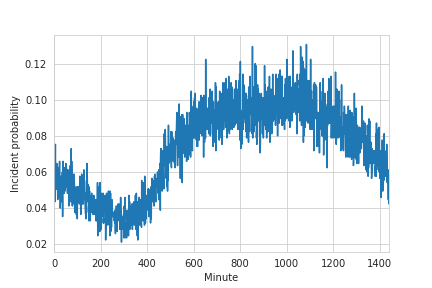
\includegraphics[width=12cm,keepaspectratio]{Figures/raw_signal.png}
  \caption{The aggregated probability of an emergency call for each of the 1,440 minutes of the day}
  \label{fig:raw_signal}
\end{figure}



\section{Modeling methodology}
\subsection{Data processing}
\subsection{Distribution fitting}
\begin{equation}
p(x) = A_0 + \sum_{n=1}^{N} A_ncos(nw_0x) + B_nsin(nw_0x)
\label{eq:fourier_poly}
\end{equation}

\subsection{Value quantification}




\section{Insights and recommendations}


\section{Conclusions and future work}




\bibliographystyle{Bibliography_Style}
\scriptsize{
\bibliography{./References}
}

\end{document}
